\chapter{Mobile Autonomous Shotcrete and Scanning System Overview}
\label{chap:overview}
\section{Chapter Overview}
\section{Design Process}
\label{sec:design}
\subsection{Customer Requirements}
There are two ``Customers'' in this research, the industry partner and the research facility. The industry partner, Cameco, requires a proof of concept prototype with functional algorithms that can be implemented in a final production model. The research facility, UOIT, requires a system on which novel software and hardware designs can be implemented and tested for academic research and publication. It is the requirement of this work to meet both customer's needs.\\

\begin{table}[h!]
\begin{adjustwidth}{-.75in}{-.25in}  
\begin{tabular}{|L{0.05\linewidth} L{0.25\linewidth}|L{0.7\linewidth}|}
\hline
\multicolumn{3}{|c|}{\textbf{Cameco Requirements}} \\ \hline
\multicolumn{2}{|c|}{Requirement} & \multicolumn{1}{c|}{Discussion} \\ \hline
R$_C$1: & Proof of concept hardware prototype & The proof of concept prototype is Cameco's way of evaluating the success of the research and determining the whether the software and hardware designs are a feasible substitute for the current practices.\\ \hline
R$_C$2: & Autonomous scanning & The robot must be able to scan the drift face for radiation with minimal input from an operator. The operator should only have to select an area to scan. \\ \hline
R$_C$3: & Autonomous shotcreting & The robot must be able to apply shotcrete with minimal input from an operator. The robot should be able to apply shotcrete autonomously once positioned or directed to the starting location. \\ \hline
R$_C$4: & Autonomous navigation & The robot must be able to navigate to the desired location with minimal input from an operator. The operator must be able to intuitively define a location to autonomously navigate to, as well as be able to manually drive the robot. \\ \hline
R$_C$5: & Obstacle avoidance & The robot must not collide with obstacles, stationary or moving, while navigating. The obstacles my appear at any time during operation.\\ \hline
R$_C$6: & Improved efficiency & The robot must be able to perform the task in equal or less time than the current standard. \\ \hline
R$_C$7: & Improved accuracy & The robot must be able to perform the task with equal or greater accuracy than the current standard. The includes the application and measurement of the shotcrete layer. \\ \hline
R$_C$8: & 3D reconstruction & Though not a requirement of the customer, in order to perform certain functions the data necessary to generate a 3D reconstruction of the mine must be obtained. The 3D mine reconstruction is an added feature to be offered to the customer, so it is treated as a requirement.\\ \hline
R$_C$9: & Worker safety & The robot must ensure workers are safe during the operation of the robot, and must also ensure the modifications to its surroundings do not increase the risk worker safety. \\ \hline
R$_C$10: & Environmental Protection & The robot must be able to function in the environmental conditions of an underground uranium drift mine. \\ \hline
\end{tabular}
\caption{Cameco Customer Requirements}
\label{tab:reqs}
\end{adjustwidth}
\end{table}
\begin{table}[h!]
\begin{adjustwidth}{-.75in}{-.25in}  
\begin{tabular}{|L{0.05\linewidth}L{0.25\linewidth}|L{0.7\linewidth}|}
\hline
\multicolumn{3}{|c|}{\textbf{UOIT Requirements}} \\ \hline
\multicolumn{2}{|c|}{Requirement} & \multicolumn{1}{c|}{Discussion} \\ \hline
R$_U$11: & Functioning prototype & To consider the design problem solved, the system must function as intended providing a novel solution to the problems outlined.\\ \hline
R$_U$12: & Accurate localization & The robot must be able to autonomously localize itself within it's environment. Testing must be performed with a ground truth system. \\ \hline
R$_U$13: & Novel design & The research must be original. \\ \hline
R$_U$14: & Use of engineering principals & Engineering principals and practices must be used in the design of the system. \\ \hline
R$_U$15: & Research oriented & The robot must prove a valuable research tool. The insight gained from the testing should have value, and the hardware prototype should continue to be a useful tool once this research completes. \\ \hline
R$_U$16: & Publications & The robot must employ novel design features with significant enough impact to the research community that can be published in academic peer reviewed publications. \\ \hline
R$_U$17: & Continuation Opportunity & The design must not be a dead-end, further opportunities for novel design implementations must be possible. Either additional hardware modifications can be made, software packages can be built, or novel analysis of the obtained data must be possible. \\ \hline
R$_U$18: & Ethical practices & The robot's intended use must be ethical. While the robot may replace human workers, the physical safety of the workers is of greater concern. No part of the design shall be built with the intention to be used in a way that can intentionally harm people, society, or the environment. \\ \hline
\end{tabular}
\caption{UOIT Customer Requirements}
\label{tab:ureqs}
\end{adjustwidth}
\end{table}
\subsection{Engineering Requirements}
\begin{table}[h!]
\begin{adjustwidth}{-.75in}{0in}  
\begin{tabular}{|L{0.05\linewidth} L{0.25\linewidth}|L{0.7\linewidth}|}
\hline
\multicolumn{2}{|c|}{Customer Requirement} & Engineering Requirements \\ \hline
R$_C$1: & Proof of concept hardware prototype & \begin{tabular}{L{0.05\linewidth} L{0.9\linewidth}}
E1: & Apply shotcrete in a timely manner\\
E2: & Scan drift face accurately\\
\end{tabular} \\ \hline
R$_C$2: & Autonomous scanning & \begin{tabular}{L{0.05\linewidth} L{0.9\linewidth}}
E3: & Position end-effector accurately for scanning\\
E4: & Record position and radiation levels accurately\\
\end{tabular} \\ \hline
R$_C$3: & Autonomous shotcreting & \begin{tabular}{L{0.05\linewidth} L{0.9\linewidth}}
E5: & Position end-effector accurately for spraying\\
E6: & Measure shotcrete thickness\\
\end{tabular} \\ \hline
R$_C$4: & Autonomous navigation & \begin{tabular}{L{0.05\linewidth} L{0.9\linewidth}}
E7: & Navigate to desired location\\
E8: & Ackerman steering for trailer\\
\end{tabular} \\ \hline
R$_C$5: & Obstacle avoidance & \begin{tabular}{L{0.05\linewidth} L{0.9\linewidth}}
E9: & Avoid obstacles by user-defined distance\\
\end{tabular} \\ \hline
R$_C$6: & Improved efficiency & \begin{tabular}{L{0.05\linewidth} L{0.9\linewidth}}
E10: & Perform scanning task faster than current practices\\
E11: & Perform shotcreting task faster than current practices\\
\end{tabular} \\ \hline
R$_C$7: & Improved accuracy & \begin{tabular}{L{0.05\linewidth} L{0.9\linewidth}}
E12: & Record radiation measurements with greater accuracy\\
E13: & Record radiation measurement positions with greater accuracy\\
E14: & Measure shotcrete thickness with greater accuracy than current practices\\
\end{tabular} \\ \hline
R$_C$8: & 3D reconstruction & \begin{tabular}{L{0.05\linewidth} L{0.9\linewidth}}
E15: & Generate registered point cloud of mine environment\\
\end{tabular} \\ \hline
R$_C$9: & Worker safety & \begin{tabular}{L{0.05\linewidth} L{0.9\linewidth}}
E16: & Minimize safety risk when present in a mine\\
\end{tabular} \\ \hline
R$_C$10: & Environmental Protection & \begin{tabular}{L{0.05\linewidth} L{0.9\linewidth}}
E17: & Reduce environmental impact\\
\end{tabular} \\ \hline
R$_U$11: & Functioning prototype & \begin{tabular}{L{0.05\linewidth} L{0.9\linewidth}}
E18: & Generate motion trajectories\\
E19: & Perform radiation scanning motions\\
E20: & Perform shotcrete application motions\\
E21: & Estimate thickness\\
\end{tabular} \\ \hline
R$_U$12: & Accurate localization & \begin{tabular}{L{0.05\linewidth} L{0.9\linewidth}}
E22: & Determine robot location\\
\end{tabular} \\ \hline
R$_U$13: & Novel design & \begin{tabular}{L{0.05\linewidth} L{0.9\linewidth}}
E$_x$: & This can not be defined explicitly as an engineering specification\\
\end{tabular} \\ \hline
R$_U$14: & Use of engineering principals & \begin{tabular}{L{0.05\linewidth} L{0.9\linewidth}}
E$_x$: & This can not be defined explicitly as an engineering specification, but includes the elements presented in the Design Process section \\
\end{tabular} \\ \hline
R$_U$15: & Research oriented & \begin{tabular}{L{0.05\linewidth} L{0.9\linewidth}}
E23: & Modular design\\
\end{tabular} \\ \hline
R$_U$16: & Publications & \begin{tabular}{L{0.05\linewidth} L{0.9\linewidth}}
E$_x$: &This can not be defined explicitly as an engineering specification. If R$_U$13 is completed and the research is worthwhile the requirement is considered fulfilled\\
\end{tabular} \\ \hline
R$_U$17: & Continuation Opportunity & \begin{tabular}{L{0.05\linewidth} L{0.9\linewidth}}
E24: & Proper documentation\\
\end{tabular} \\ \hline
R$_U$18: & Ethical practices & \begin{tabular}{L{0.05\linewidth} L{0.9\linewidth}}
E25: & Adhere to ethical standards throughout design process\\
\end{tabular} \\ \hline
\end{tabular}
\caption{UOIT Customer Requirements}
\label{tab:ureqs}
\end{adjustwidth}
\end{table}
\subsection{House of Quality}
\subsection{Project Resources}
\subsection{Project Methodology}
\subsection{Engineering Targets}
\subsection{Concept Generation}
\subsection{Concept Evaluation}
\subsection{Failure Mode and Effect Analysis}
\section{Hardware}
\subsection{Husky}
\begin{figure}[H]
    \centering
    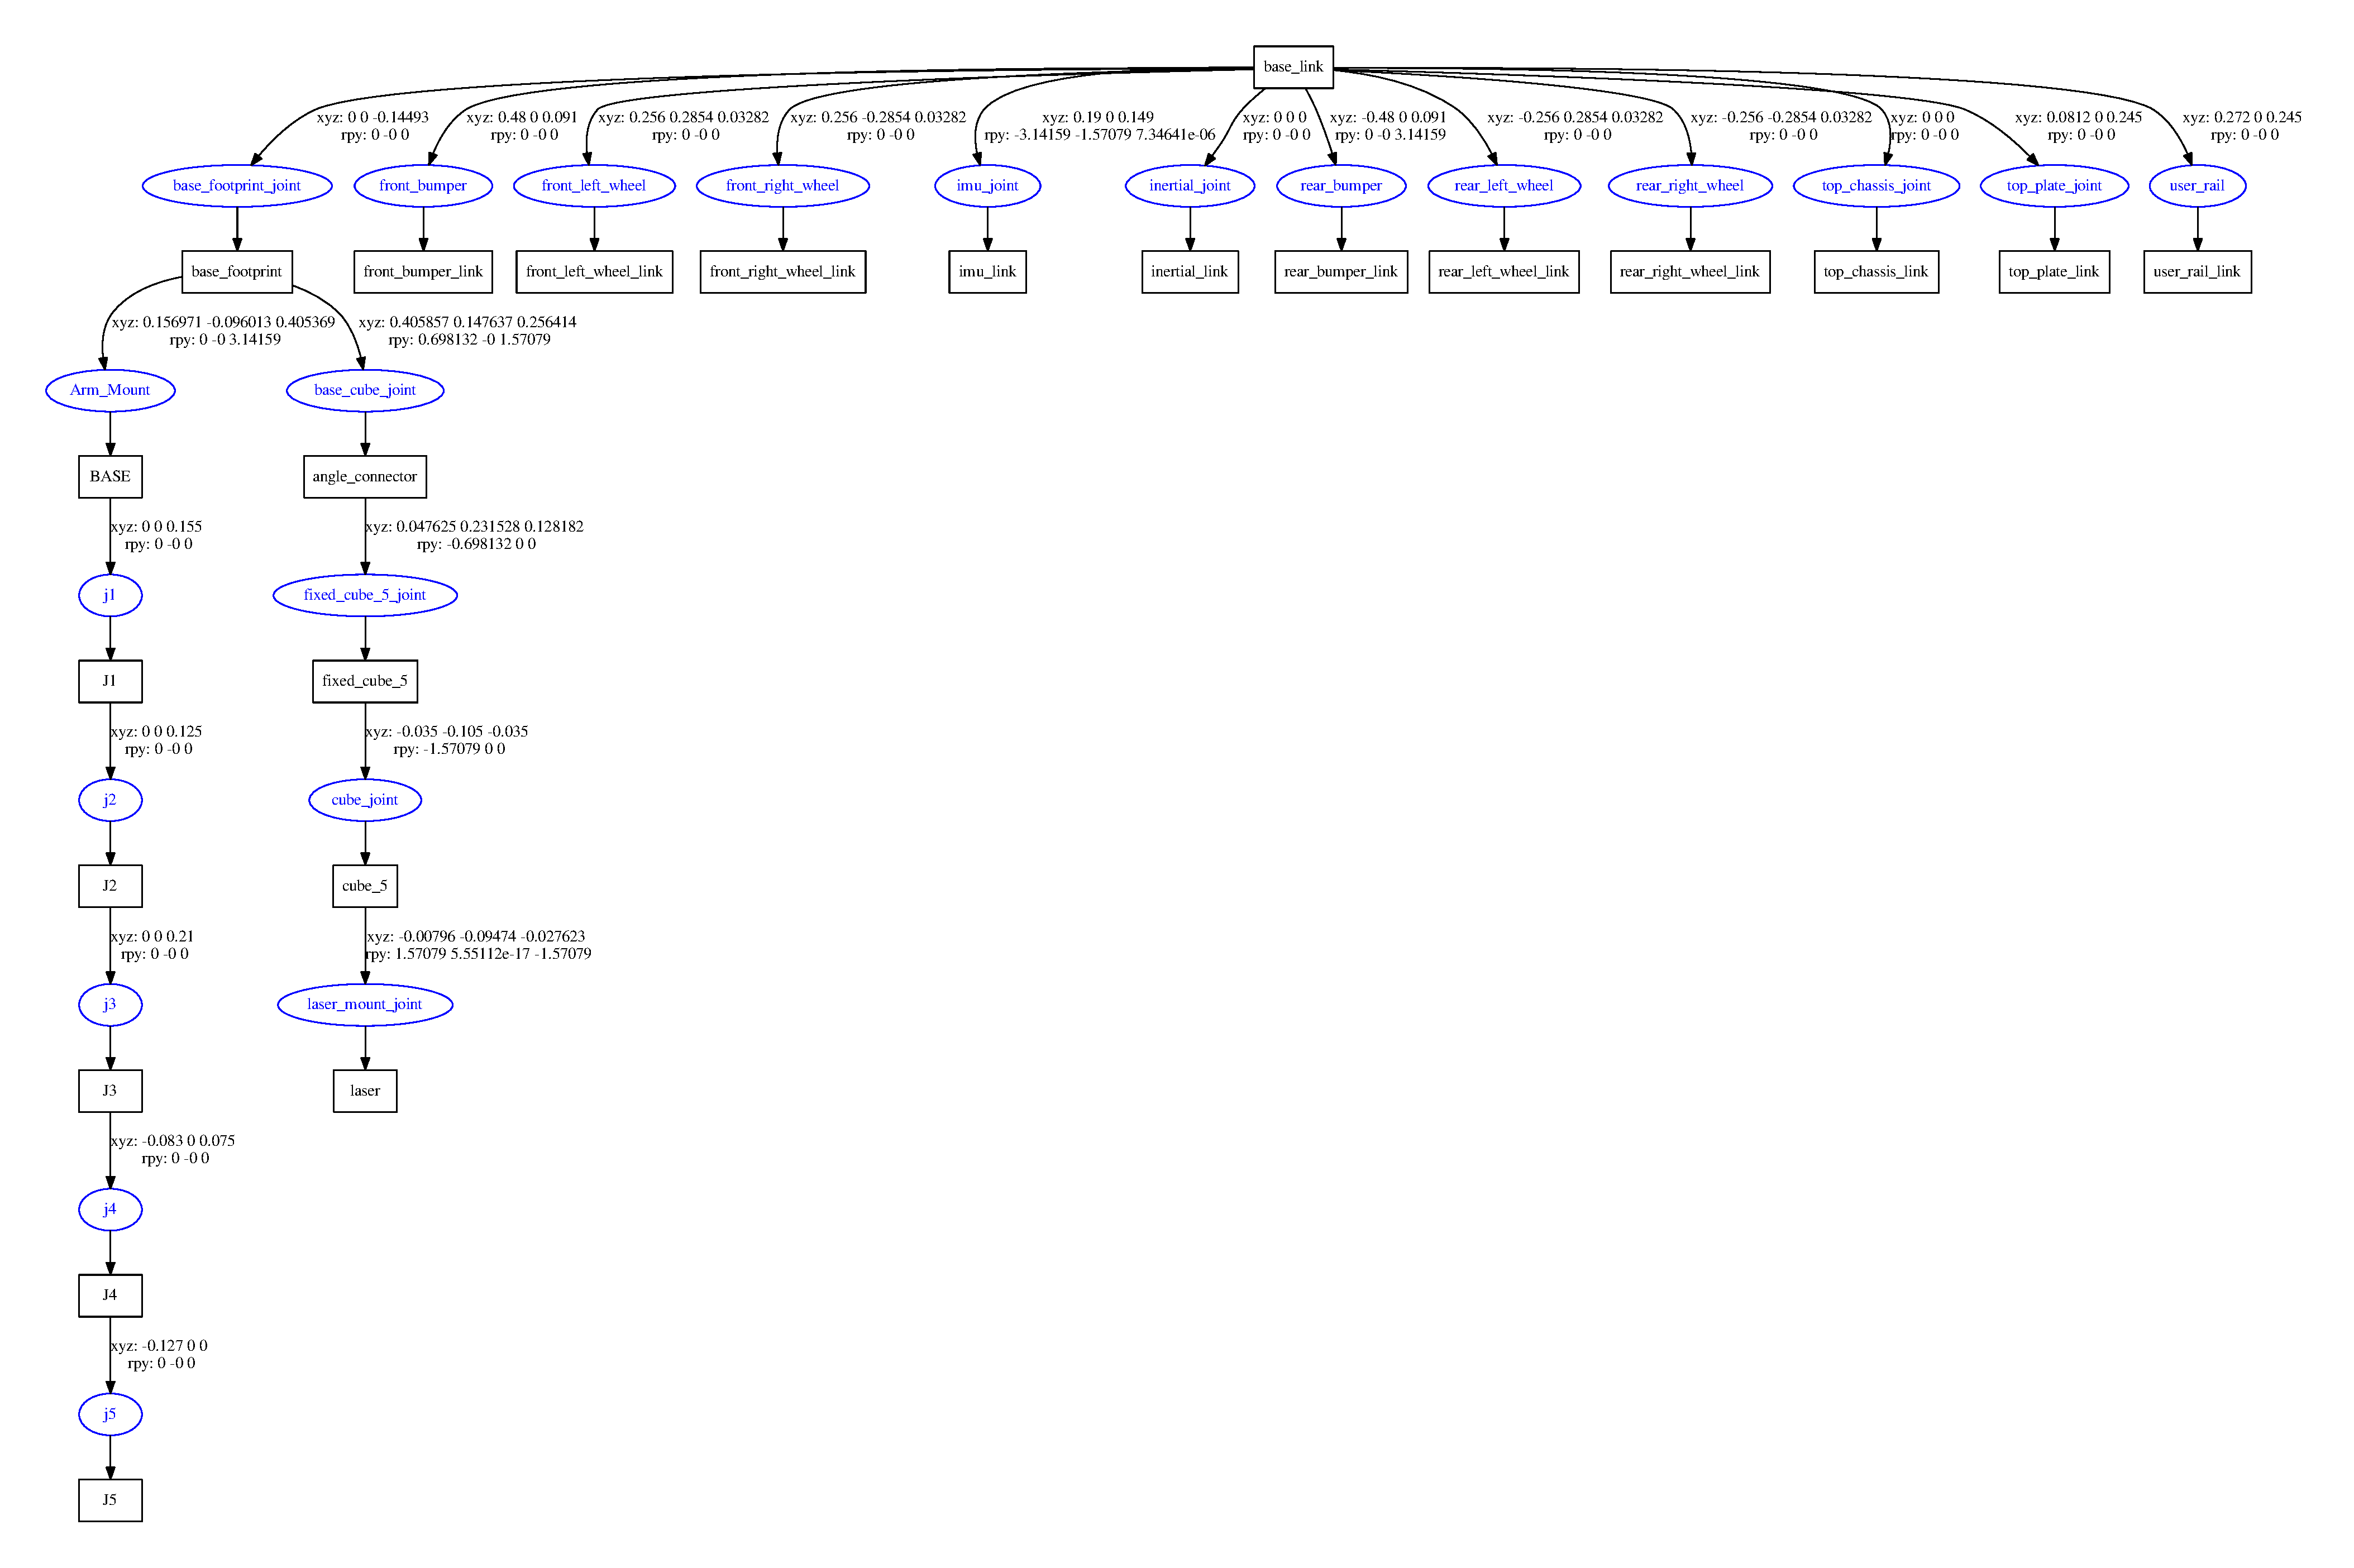
\includegraphics[width=0.8\textwidth]{Pics/husky.jpg}
    \caption{Husky UGV \cite{huskypage}}
    \label{fig:husky}
\end{figure}
%https://www.clearpathrobotics.com/husky-unmanned-ground-vehicle-robot/
Clearpath's Husky Unmanned Ground Vehicle (Husky UGV) is the mobile base used for the proof of concept prototype. It is a four wheeled skid steer vehicle, capable of driving on uneven ground or loose gravel. It has a wheel diameter of 330mm, and external dimensions of 990mm $\times$ 670mm $\times$ 390 mm. It's maximum payload is 75kg and maximum speed is 1.0 m/s. Skid steer vehicles have notoriously unreliable odometry data which makes the Husky an excellent choice as a mobile base, since it creates a more realistic representation of the final product.\\
\subsection{Husky Peripherals}

\begin{figure}[H]
    \centering
    \includegraphics[width=\textwidth]{Pics/DSC0433.JPG}
    \caption{Husky With Peripherals Attached}
    \label{fig:peripherals}
\end{figure}
The Husky required a few modifications to support the additional hardware used. A top plate was machined to mount the manipulator, as well as a mounting bracket for the nodding head servo. A trailer hitch was installed and a trailer was built to allow the Husky to tow additional batteries, a generator, and the controller for the manipulator.\\
\subsection{DENSO VP6242}
\begin{figure}[H]
    \centering
    \includegraphics[width=0.6\textwidth]{Pics/denso.png}
    \caption{DENSO VP6242 Manipulator \cite{densopage}}
    \label{fig:sick}
\end{figure}
%https://www.denso-wave.com/en/robot/product/five-six/vp.html
The final product will likely use hydraulics to position the shotcreting and scanning end-effector since the payload and forces will require a high strength and rigidity manipulator. Designing a manipulator for this task is outside the scope of this research, so a suitable analogue was chosen. The requirements of the manipulator is that it can position it's end-effector with 6 Degrees-of-Freedom like the final version, but does not require the same workspace, strength, or rigidity the final product would in order to accurately position the end-effector and apply shotcrete. The DENSO manipulator was chosen since it fulfils all the application requirements and was available at UOIT for use in this work. It has a maximum reach of 432mm and a maximum payload of 2.5kg.\\ 
\subsection{LMS101}

\begin{figure}[H]
    \centering
    \includegraphics[width=0.4\textwidth]{Pics/sick.png}
    \caption{SICK LMS101 LIDAR \cite{sickpage}}
    \label{fig:sick}
\end{figure}
%https://www.sick.com/de/en/detection-and-ranging-solutions/2d-lidar-sensors/lms1xx/lms101-10000/p/p346868?ff_data=JmZmX2lkPXAzNDY4NjgmZmZfbWFzdGVySWQ9cDM0Njg2OCZmZl90aXRsZT1MTVMxMDEtMTAwMDAmZmZfcXVlcnk9JmZmX3Bvcz04JmZmX29yaWdQb3M9OCZmZl9wYWdlPTEmZmZfcGFnZVNpemU9OCZmZl9vcmlnUGFnZVNpemU9OCZmZl9zaW1pPTkzLjA=
The LMS101 is a LIDAR scanner manufactured by SICK. It has an aperture angle of 270$\degree$, angular resolution of 0.25$\degree$ at 25Hz, and optimal range of 0.5m-20m. SICK is a well know brand of LIDAR scanners, with lots of software drivers available for the various systems it works with. The ROS driver for this LIDAR does not natively support 0.25$\degree$ resolution, so it has been modified accordingly. It has a systematic error of $\pm$30mm and statistical error	of 12mm, though through testing it was found the LIDAR performs much better in the given test conditions. With and IP rating of IP65, it is suitable for indoor use but can be replaced with another model from the same family with equal performance but higher IP rating (up to IP67).\\
\subsection{Schunk Powercube PR70}
\begin{figure}[H]
    \centering
    \includegraphics[width=0.5\textwidth]{Pics/powercube.png}
    \caption{Schunk Powercube PR70 \cite{schunkpage}}
    \label{fig:schunk}
\end{figure}
%https://www.comoso.com/uploads/products/downloads/Schunk_Comoso_PR_gesamt_EN.pdf
The LIDAR must be mounted on a nodding head to produce pointclouds. The Powercube PR70 made by Schunk was chosen for this task partly since it was already an asset of the UOIT MARS lab. The module has higher accuracy and payload than the application requires, but since it was an unused asset it was chosen for this application minimize budgetary impact. It has a nominal torque of 15Nm, repeat accuracy of 0.03$\degree$, maximum angular velocity of 240$\degree$/s, and maximum acceleration of 960$\degree$/s$^2$. \\
\section{Software}
\label{sec:software}
All software integrated and developed for this research is intended for use within the ROS framework. Since ROS is an open source community with many packages available for use in research, it offers a wide selection of resources useful to this work. The framework itself was designed for modularity and functionality with robotics, making it an excellent choice for use in this work.\\
\subsection{Overview of the Existing ROS Packages used}

Many of the tasks required for operation of the MASSS have already been developed by the ROS community. Hardware drivers, motion controllers, LIDAR scan to pointcloud assemblers, navigation, and mapping packages are already available through the ROS website. An engineer's job is not to ``reinvent the wheel'', so software that has already been developed that is applicable to this system was used.\\
\subsubsection{RVIZ}
\label{sec:rviz}

Documentation on RVIZ can be found at \url{http://wiki.ros.org/rviz}\\

RVIZ is a powerful visualization tool developed for use with ROS. There is a large quantity of information that can be generated using ROS that is not easily interpreted without the use of an interactive graphical user interface. RVIZ allows users to view, interact with, interpret, and modify the data handled within ROS. RVIZ is an invaluable tool in mobile robotics; it can display a model of the robot, a map the robot has generated of its environment, the path it intends to follow, and display sensor data the robot acquires. The user can interact with RVIZ and send commands to the robot like position goals, movement commands, status changes, or selecting parts of the sensor data to be used in other software controls algorithms.\\

RVIZ is designed to be adaptable for whatever the operator needs. Custom tools and plugins are easily developed to make RVIZ helpful in the context it is used. In this work, a custom tool was implemented for selecting sections of the mine surface to be scanned or shotcreted. A custom plugin called the control panel was created to provide the user with a user-friendly interface to command and control all relevant aspects of the MASSS.\\

RVIZ configurations can be saved to a file and loaded at launch when the robot control system is brought online. The configuration file for this work sets the RVIZ environment in a way that is functional for the operator, but includes options to reveal information important for debugging and research. For example, under most circumstances the pointcloud representation of the mine surface should be shown but the individual laser scans are hidden. If the operator wanted to see the instantaneous view of the robot's environment represented as a laser scan, the topic's checkbox simply needs to be checked. Similarly, pointclouds are cropped to remove sections of the robot detected be the scanner but can be visualized by enabling the appropriate display. When generating trajectories the surface path, surface normals, and end-effector path is shown, however the operator may only want some or none of the information displayed so they are all easily hidden or shown.\\

\subsubsection{Husky}

Documentation of the Husky package can be found at \url{http://wiki.ros.org/Robots/Husky}\\

The Husky package is made by Clearpath Robotics to provide ROS functionality to their Husky Unmanned Ground Vehicle (UGV). The package consists of the following subpackages:

\begin{itemize}
    \item husky\_base
    \item husky\_bringup
    \item husky\_gazebo
    \item husky\_viz
    \item husky\_control
    \item husky\_description
    \item husky\_msgs
    \item husky\_navigation
\end{itemize}

\paragraph{husky\_base}

The husky\_base package provides the low level communication between ROS and the robot. It contains all the necessary drivers to allow the robot to operate under ROS control.\\

\paragraph{husky\_bringup}

The husky\_bringup package contains a number of scripts to that launch all the necessary packages (like husky\_base) for the robot to function. Many applications for the Husky robot are intended to be turnkey, so the bringup package allows the designer to set what packages to launch when the robot boots up. Using the bringup package the robot can be configured to commence its control system as soon as it is powered on.\\

\paragraph{husky\_gazebo}

Gazebo is a simulation tool used in ROS. With a fully defined robot model, Gazebo can simulate the robot in a user defined environment. If an operator intends to test their algorithms on a Husky robot, but does not have access to a physical robot they can test their software our on a simulated version of the Husky. Similarly, if the operator wants to test their robot in a scenario that may cause damage to the robot, or in an environment they are unable to create, they can use Gazebo to test their algorithms in simulation.\\

\paragraph{husky\_viz}

As mentioned in \ref{sec:rviz}, RVIZ configurations can be saved and loaded by ROS. The husky\_viz package contains various configurations for RVIZ that optimize its configuration for use with the Husky.\\

\paragraph{husky\_control}

husky\_control turns motion goals in to actual robot motion. The motion goals are published using ROS topics, and the husky\_control package subscribes to these topics and moves the robot accordingly. The motion goals can be provided directly from the operator using an input device such as a joystick, or generated from autonomous navigation packages acting on a goal location provided by the operator. The source of the motion commands does not affect how the package functions, so it is able to receive motion command from a wide variety of sources as long as the commands are formatted using the appropriate ROS message type.\\ 

\paragraph{husky\_description}

In order to visualize the robot in the RVIZ environment, the robot requires a description. The robot description contains all the relevant information about the robot parts, which way they can move, what colour they are, and how to visually represent them. The description also contains the relevant physical characteristics to simulate the robot in Gazebo. The husky\_description package uses the Unified Robot Description Format (URDF) to describe the model for the Husky UGV.\\

\paragraph{husky\_msgs}

To communicate with other packages, or within the Husky packages, custom messages for the Husky robot are used. The husky\_msgs package contains these custom messages. An example of the HuskyStatus message can be found in Appendix \ref{app:huskystatus}

%\includecode[pythonstyle]{Code/HuskyStatus.msg}{HuskyStatus.msg}

\paragraph{husky\_navigation}

The husky\_navigation package provides configurations and examples for using varous navigation packages with the Husky. It contains all the relevant information a navigation package requires to successfuly apply the navigation algorithm on the Husky. Things like the robot's footprint size, how far away to stay from obstacles, what sort of behaviours to exhibit when encountering obstacles, and what sensor information is available are contained within the configuration files. Navigation packages require the configurations for their global and local planners that is contaoned within the husky\_navigation package. The configuration file for producing costmaps for use in navigation is shown in Appendix \ref{app:huskyconfig} to provide an example of what the configuration files look like.\\

The package contains launch files to use various navigation packages with the Husky robot as well as demos that will launch the required accompanying packages as well. Launch files for AMCL, Gmapping, Frontier Exploration, and Move Base packages are included, as well as an empty map for use when the robot is being simulated in Gazebo.\\ 

\subsubsection{Move Base}

Documentation of the Move Base package can be found at \url{http://wiki.ros.org/move_base}\\

\begin{figure}[H]
    \centering
    \includegraphics[width=\textwidth]{Pics/overview_tf.png}
    \caption{Overview of the Move Base Package \cite{rosmovebase}}
    \label{fig:movebaseoverview}
\end{figure}

The move\_base package takes high level commands like a location goal and performs the necessary actions to drive the robot to that location, a graphical overview of the package is shown in figure \ref{fig:movebaseoverview}. It divides the task among two planners, the global planner and the local planner. The global planner is responsible for creating the overall plan for the robot path. It uses a global costmap generated by the map server, which holds the map generated by the SLAM algorithm or loaded from file. The global costmap includes things like the inflation layer, which acts as a safety buffer by creating a region surrounding any obstacles within the map that the robot cannot enter. The local costmap is generated based on what the robot's sensors currently detect. If a person were to walk in front of the robot, they would appear in the local costmap and the local planner would generate a path around the obstacle attempting to continue along the path generated by the global planner. If, for example, a person or object is placed close enough to the robot that it ends up occupying the space created by the inflation layer of the obstacle it becomes stuck. Once stuck, the robot must execute recovery behaviours to become unstuck. Figure \ref{fig:recovery} shows what recovery behaviours move\_base attempts to free itself. First the robot deletes obstacles from the map that are further away than a user specified distance. If the robot is then free to move, it will continue its navigation. If the robot is still stuck, it will rotate on the spot to get an updated view of its surroundings. If it still cannot move it will clear the map of all obstacles that are not within the area it needs to rotate in place, and if still stuck will rotate once more to scan its environment for obstacles. Once the second clearing rotation is complete if it is still unable to move it will abort its current goal and release a message notifying the system it was unable to reach its target location.\\

\begin{figure}[H]
    \centering
    \includegraphics[width=\textwidth]{Pics/recovery_behaviors.png}
    \caption{Move Base Recovery Behaviours \cite{rosmovebase}}
    \label{fig:recovery}
\end{figure}

\subsubsection{Laser Assembler}


Documentation of the Laser Assembler package can be found at \url{http://wiki.ros.org/laser_assembler}\\

The laser\_assembler package converts the stream of laserscan data to a pointcloud. When the system creates a pointcloud representation of it's surroundings, it tells the laser\_assembler package when to start and stop recording the laser scans generated by the LMS100 LIDAR scanner. The assembler will store all of the laserscans, along with the coordinate frame transformation from a fixed frame to the LIDAR frame at that moment. When the pointcloud scan is complete, the laser\_assembler is notified and produces a pointcloud in the coordinate frame requested by the user. Discussed further in Section \ref{sec:locsourceerror}, the parameter ``ignore\_laser\_skew'' is set to false so that each point in the laser scan is transformed using the current pose of the LIDAR rather than the whole scan at once.\\

\subsubsection{Hector SLAM}

Documentation of the Hector SLAM package can be found at \url{http://wiki.ros.org/hector_slam}\\

The hector\_slam package contains the hector\_mapping package used by the MASSS to perform SLAM. The two main SLAM packages available for use with ROS are Gmapping and Hector SLAM. Gmapping is a more popular algorithm, but requires odometry from the robot. Hector SLAM can perform SLAM without the need for odometry. While the MASSS does measure its odometry, it is intended for use on uneven rocky ground and odometry may not be reliable. For that reason, Hector SLAM was chosen as the SLAM algorithm for use on the MASSS. However, thanks to the modularity that ROS offers it is a simple task to utilize other SLAM algorithms like Gmapping on the MASSS.\\

\subsubsection{RQT Reconfigure}

Documentation of the RQT Reconfigure package can be found at \url{http://wiki.ros.org/rqt_reconfigure}\\

If a node has been configured with parameters that can change at runtime, \node{rqt_reconfigure} can be used to modify them. When the user launches the GUI, it will poll the ROS parameter server to determine which nodes have dynamically reconfigurable variables and what their values and acceptable ranges are. I then presents the user with a window that shows a list of nodes on the left. When a node is selected the configurable parameters are shown on the right, most often in the form of a slider bar. An example \node{rqt_reconfigure} GUI window can be seen in figure \ref{fig:dyngui2}.

\begin{figure}[h]
    \centering
    \includegraphics[width=0.8\textwidth]{Pics/dyngui.png}
    \caption{\texttt{rqt\_reconfigure} GUI}
    \label{fig:dyngui2}
\end{figure}

\subsection{Overview of the MASSS ROS Package}
\label{sub:software}

A thorough discussion of the source code is provided in Chapter \ref{chap:code}, however an overview of the MASSS would be incomplete without mentioning the ROS package that provides its functionality. The complete code can be found in Appendix \ref{app:code}.\\ 

The main interface between the user and the control system occurs within an RVIZ window. Along with the regular features of RVIZ, this software adds a panel and a tool to the RVIZ interface. The additional features can be seen in Figure \ref{fig:panel}. The code for the control panel is split between two files. For the system's current purpose it would be far less functional to have a standalone Graphical User Interface (GUI) and not use RVIZ for visualization therefore \node{control_dashboard} was designed as a plugin for RVIZ. As future work on this project continues, the need for RVIZ visualization may diminish, so the node was designed to make converting it to run without RVIZ a trivial task. Eventually, when this system is implemented in a mine, no graphical interface at all will be required on the machine itself. For that reason, the core functionality of the system lies in the \node{control_panel} node. The \node{control_dashboard} node simply relays the actions in the user interface to the \node{control_panel} node.\\

The \node{control_panel} node is the heart of the control system. It is responsible for calling the localization, trajectory generation, and thickness estimation services, as well as communication with the DENSO arm, PowerCube servo, and Husky UGV. Other tasks specific to the MASSS requirements such as modifying trajectory points to fit within the DENSO arm's workspace are performef be \node{control_panel}. As well, the parts of the robot visible to the laser scanner that may be interpreted as part of the environment are cropped.\\

The main contribution to the ROS community are the localization, trajectory generation, and thickness estimation services. These three services are intended to be as portable as possible so they can be useful in any robotics project, regardless of the system configuration. Should other researchers have a need for a service they can provide, one simply needs to install the package and will be able to launch the desired service from the terminal or their own launch file. Unfortunately, due to this document's confidentiality the source code will not be made available, so the functionality of the compiled binaries are provided as-is.\\


